\documentclass[11pt,a4paper]{article}
\usepackage[T1]{fontenc}
\usepackage[utf8]{inputenc}
\usepackage[margin=23mm,headheight=15pt]{geometry}
\usepackage{amsmath,amssymb,mathtools,amsthm}
\usepackage{newpxtext,newpxmath}
\usepackage{microtype,xcolor,enumitem,environ,needspace,fancyhdr,etoolbox}
\usepackage{tikz}
\usetikzlibrary{arrows.meta}
\usepackage[colorlinks=true,linkcolor=heading,urlcolor=heading]{hyperref}
\definecolor{heading}{HTML}{244B65}
\definecolor{hintcolor}{HTML}{765638}
\definecolor{sourcecolor}{HTML}{C74743}
\definecolor{targetcolor}{HTML}{2878B5}
\definecolor{mapcolor}{HTML}{77529B}
\tikzset{
  exo axis/.style={draw=gray!75,thin,-{Stealth[length=1.5mm]}},
  exo guide/.style={gray!50,thin,dashed},
  exo source/.style={sourcecolor,line width=1.1pt},
  exo target/.style={targetcolor,line width=1.1pt},
  exo map/.style={mapcolor,line width=1.2pt},
  exo arrow/.style={mapcolor,line width=.8pt,-{Stealth[length=1.6mm]}}
}
\setlength{\parindent}{0pt}
\setlength{\parskip}{5pt plus 1pt}
\setlength{\emergencystretch}{2em}
\setlist{topsep=4pt,itemsep=4pt,parsep=2pt,leftmargin=*}
\allowdisplaybreaks[1]
\newtheoremstyle{exostyle}{8pt}{6pt}{\normalfont}{}{\color{heading}\bfseries}{.}{\newline}{}
\theoremstyle{exostyle}
\newtheorem{exercise}{Exercise}
\BeforeBeginEnvironment{exercise}{\par\addvspace{10pt}\Needspace{9\baselineskip}%
  \begingroup\color{heading!45}\hrule height .6pt\endgroup\nobreak}
\newif\ifcorr
\ifdefined\StatementOnly\corrfalse\else\corrtrue\fi
\newcommand{\showsolutions}{\corrtrue}
\newcommand{\hidesolutions}{\corrfalse}
\NewEnviron{hints}{\ifcorr\par\Needspace{4\baselineskip}\noindent
  {\color{hintcolor}\bfseries Useful hints}\par\BODY\par\medskip\fi}
\NewEnviron{solution}{\ifcorr\par\Needspace{4\baselineskip}\noindent
  {\color{heading}\bfseries Detailed solution}\par\BODY\par\medskip\fi}
\newcommand{\R}{\mathbb{R}}
\newcommand{\push}{\#}
\newcommand{\W}{\mathcal{W}}
\newcommand{\Wone}{\mathcal{W}_1}
\newcommand{\Wtwo}{\mathcal{W}_2}
\newcommand{\Unif}{\mathcal U}
\newcommand{\ip}[2]{\langle #1,#2\rangle}
\newcommand{\gradW}{\mathord{\nabla\mkern-9.3mu\nabla}}
\pagestyle{fancy}
\fancyhf{}
\fancyhead[L]{\small\color{heading}Optimal Transport / Exercises}
\fancyhead[R]{\small\ifcorr Solutions\else Statements\fi}
\fancyfoot[C]{\small\thepage}
\renewcommand{\headrulewidth}{0.3pt}
\renewcommand{\maketitle}{\thispagestyle{plain}\begingroup
  \color{heading}\LARGE\bfseries\SheetTitle\par\endgroup
  \vspace{3pt}{\large\ifcorr Statements, hints and worked solutions\else Exercise statements\fi}\par
  \vspace{7pt}\hrule\vspace{9pt}
  \ifcorr Each exercise is followed by question-by-question hints and a worked solution.
  Try the questions before reading the hints.\else
  This version contains the exercises only. Hints and worked solutions are available in the companion PDF.\fi
  \par\medskip}
\hypersetup{pdfauthor={Optimal Transport for Machine Learners},pdfsubject={Exercises in optimal transport}}

\newcommand{\SheetTitle}{Monge Formulation}
\hypersetup{pdftitle={Monge Formulation -- Exercises}}
\begin{document}

\maketitle

\begin{exercise}[Discrete assignment]\label{ex:assignment}
Let $n=3$ and
$
C \;=\;
\begin{pmatrix}
2 & 1 & 3\\
3 & 2 & 2\\
4 & 3 & 1
\end{pmatrix}.
$
Identify every optimal assignment.
\end{exercise}
\begin{hints}
Enumerate the six permutations of $\{1,2,3\}$ and sum one matrix entry per row and column.
\end{hints}
\begin{solution}
For a permutation $\sigma$, the cost is $C(1,\sigma(1))+C(2,\sigma(2))+C(3,\sigma(3))$.
The minimum is $5$, achieved by the two assignments
\[
(1\!\to\!1,\;2\!\to\!2,\;3\!\to\!3)\quad\text{and}\quad
(1\!\to\!2,\;2\!\to\!1,\;3\!\to\!3).
\]
All others have cost $7$ or $9$.
\end{solution}

\begin{exercise}[Two points to two points: when does each permutation win?]\label{ex:two-points}
Fix $x_1,y_1,y_2\in\R^d$ with $y_1\ne y_2$ and let $x_2=z\in\R^d$ vary. With quadratic cost $c(x,y)=\|x-y\|^2$, compare the two assignments
\[
\text{Id: } x_1\mapsto y_1,\; z\mapsto y_2
\qquad\text{vs}\qquad
\text{Swap: } x_1\mapsto y_2,\; z\mapsto y_1.
\]
Show that the set of $z$ where \textnormal{Id} is no more expensive than \textnormal{Swap} is a half-space bounded by a hyperplane orthogonal to $y_1-y_2$. Give the equation of this hyperplane and explain that it divides $\R^d$ into two regions, one for each optimal permutation.
\begin{center}
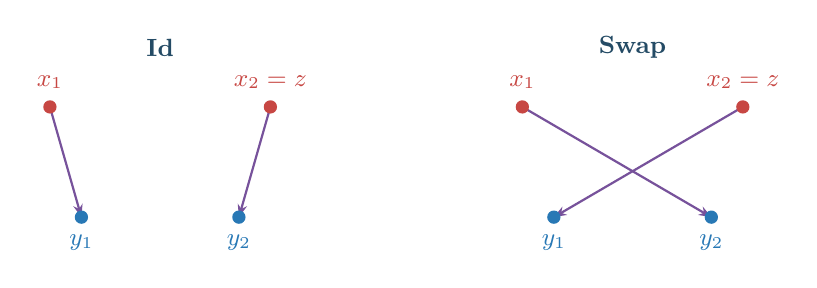
\begin{tikzpicture}[font=\small]
  \foreach \shift/\title in {0/Id,6/Swap}{
    \begin{scope}[xshift=\shift cm]
      \node[font=\small\bfseries,text=heading] at (1.4,2.15) {\title};
      \coordinate (a) at (0,1.4); \coordinate (b) at (2.8,1.4);
      \coordinate (c) at (.4,0); \coordinate (d) at (2.4,0);
      \ifnum\shift=0
        \draw[exo arrow] (a)--(c); \draw[exo arrow] (b)--(d);
      \else
        \draw[exo arrow] (a)--(d); \draw[exo arrow] (b)--(c);
      \fi
      \fill[sourcecolor] (a) circle (2.4pt) node[above=3pt] {$x_1$};
      \fill[sourcecolor] (b) circle (2.4pt) node[above=3pt] {$x_2=z$};
      \fill[targetcolor] (c) circle (2.4pt) node[below=3pt] {$y_1$};
      \fill[targetcolor] (d) circle (2.4pt) node[below=3pt] {$y_2$};
    \end{scope}
  }
\end{tikzpicture}
\end{center}
\end{exercise}
\begin{hints}
Expand the difference of the two costs; the terms $\|z\|^2$ and the target squared norms cancel.
\end{hints}
\begin{solution}
The two total costs differ by
\[
\mathrm{Id}(z)-\mathrm{Swap}(z)=2\langle z-x_1,y_1-y_2\rangle.
\]
Thus Id is optimal when $\langle z-x_1,y_1-y_2\rangle\le0$, Swap is optimal when this quantity is nonnegative, and both tie on the hyperplane
$\{z:\langle z-x_1,y_1-y_2\rangle=0\}$. Strict inequalities give strict preference. The assumption $y_1\ne y_2$ ensures this is a genuine hyperplane; if $y_1=y_2$, both assignments always tie.
\begin{center}
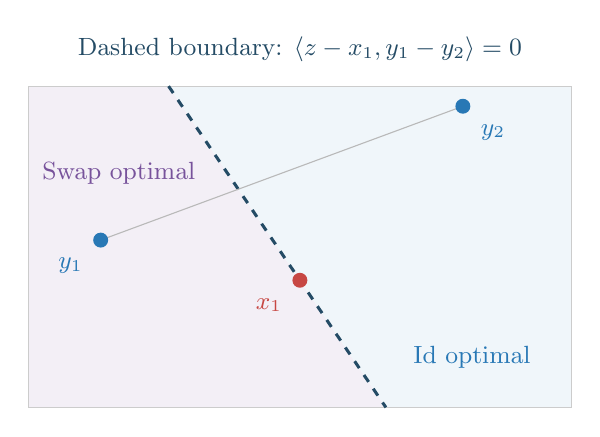
\begin{tikzpicture}[font=\small,x=1.15cm,y=.85cm]
  \fill[mapcolor!9] (-3,-2.3)--(-3,2.5)--(-1.45,2.5)--(.95,-2.3)--cycle;
  \fill[targetcolor!7] (-1.45,2.5)--(3,2.5)--(3,-2.3)--(.95,-2.3)--cycle;
  \draw[gray!40] (-3,-2.3) rectangle (3,2.5);
  \draw[heading,dashed,line width=1.1pt] (-1.45,2.5)--(.95,-2.3);
  \draw[gray!55] (-2.2,.2)--(1.8,2.2);
  \fill[sourcecolor] (0,-.4) circle (2.7pt) node[below left=3pt] {$x_1$};
  \fill[targetcolor] (-2.2,.2) circle (2.7pt) node[below left=3pt] {$y_1$};
  \fill[targetcolor] (1.8,2.2) circle (2.7pt) node[below right=3pt] {$y_2$};
  \node[text=mapcolor] at (-2,1.2) {Swap optimal};
  \node[text=targetcolor] at (1.9,-1.55) {Id optimal};
  \node[text=heading] at (0,3.05) {Dashed boundary: $\langle z-x_1,y_1-y_2\rangle=0$};
\end{tikzpicture}
\end{center}
\end{solution}

\begin{exercise}[Discrete $\to$ continuous and continuous $\to$ discrete]\label{ex:disc-cont}
(1) In 1D let $\alpha=\sum_{i=1}^N a_i\,\delta_{x_i}$ (finite support) and let $\beta$ be absolutely continuous. Show that there is no measurable map $T$ with $T_{\push}\alpha=\beta$.\\[2pt]
(2) Conversely, let $\alpha$ be absolutely continuous on $\R$ and let $\beta=\sum_{j=1}^M b_j\,\delta_{y_j}$ with $\sum_j b_j=1$. Build maps $T$ (many, up to $\alpha$-a.e. equality, if $\beta$ has at least two distinct atoms of positive mass) with $T_{\push}\alpha=\beta$.\\[2pt]
(3) Let $\alpha=\Unif[0,1]$ and let $\beta=\sum_{j=1}^M b_j\,\delta_{y_j}$ on $\R$ with $b_j>0$, $\sum_j b_j=1$, and $y_1<\cdots<y_M$. For $p\ge1$, compute an $\W_p$-optimal Monge map $T:[0,1]\to\R$ from $\alpha$ to $\beta$.\\[2pt]
(4) Suppose $b_j=1/n$ for $j=1,\dots,n$ and $y_j=\frac{j-1/2}{n}$ (midpoints of the $n$ equal subintervals of $[0,1]$). Compute $W_2^2(\alpha,\beta)$.
\begin{center}
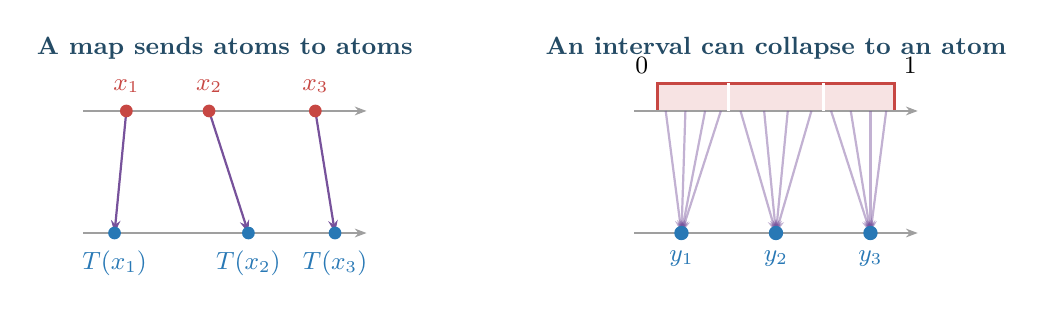
\begin{tikzpicture}[font=\small]
  \node[text=heading,font=\small\bfseries] at (1.5,2.35) {A map sends atoms to atoms};
  \draw[exo axis] (-.3,1.55)--(3.3,1.55);
  \draw[exo axis] (-.3,0)--(3.3,0);
  \foreach \x/\y/\i in {.25/.1/1,1.3/1.8/2,2.65/2.9/3}{
    \draw[exo arrow] (\x,1.55)--(\y,0);
    \fill[sourcecolor] (\x,1.55) circle (2.3pt) node[above=3pt] {$x_\i$};
    \fill[targetcolor] (\y,0) circle (2.3pt) node[below=3pt] {$T(x_\i)$};
  }
  \begin{scope}[xshift=7cm]
    \node[text=heading,font=\small\bfseries] at (1.5,2.35) {An interval can collapse to an atom};
    \fill[sourcecolor!15] (0,1.55) rectangle (3,1.9);
    \draw[exo source] (0,1.55)--(0,1.9)--(3,1.9)--(3,1.55);
    \draw[exo axis] (-.3,1.55)--(3.3,1.55);
    \draw[exo axis] (-.3,0)--(3.3,0);
    \foreach \x in {.1,.35,.6,.8}{\draw[exo arrow,opacity=.45] (\x,1.55)--(.3,0);}
    \foreach \x in {1.05,1.35,1.65,1.95}{\draw[exo arrow,opacity=.45] (\x,1.55)--(1.5,0);}
    \foreach \x in {2.2,2.45,2.7,2.9}{\draw[exo arrow,opacity=.45] (\x,1.55)--(2.7,0);}
    \foreach \x in {.9,2.1}{\draw[white,line width=1pt] (\x,1.55)--(\x,1.9);}
    \foreach \x/\i in {.3/1,1.5/2,2.7/3}{
      \fill[targetcolor] (\x,0) circle (2.6pt) node[below=3pt] {$y_\i$};
    }
    \node[above left] at (0,1.9) {$0$}; \node[above right] at (3,1.9) {$1$};
  \end{scope}
\end{tikzpicture}
\end{center}
\end{exercise}
\begin{hints}
\begin{enumerate}[label=(\arabic*)]
\item A pushforward cannot split the mass of an atom.
\item Partition the source into measurable sets with masses $b_j$; quantiles provide one such partition.
\item The interval sent to $y_j$ must have length $b_j$. Use increasing rearrangement; uniqueness need not hold when $p=1$.
\item Compute the squared distance to the midpoint in one cell, then multiply by $n$.
\end{enumerate}
\end{hints}
\begin{solution}
\emph{(1) No map from discrete to continuous.}
If $\alpha=\sum_{i=1}^N a_i\,\delta_{x_i}$ and $T$ is measurable, then
$T_{\push}\alpha=\sum_{i=1}^N a_i\,\delta_{T(x_i)}$, which is purely atomic; it cannot equal an absolutely continuous $\beta$.

\emph{(2) Many maps from continuous to discrete.}
Let $\alpha$ be absolutely continuous and $\beta=\sum_{j=1}^M b_j\,\delta_{y_j}$. Choose any measurable partition $\{A_j\}_{j=1}^M$ with $\alpha(A_j)=b_j$ (e.g.\ cut by quantiles) and set $T=\sum_{j=1}^M y_j\,\mathbf 1_{A_j}$. Then $T_{\push}\alpha=\beta$. Partitions differing on a set of positive $\alpha$-mass give distinct maps when the target has at least two distinct positive-mass atoms. A one-atom target forces the constant map.

\emph{(3) Optimal map from $\Unif[0,1]$ to a discrete law.}
Let $F_\alpha(x)=x$ on $[0,1]$ and $F_\beta$ be the CDF of $\beta$, with partial sums $s_j=\sum_{k=1}^j b_k$ and $s_0=0$. The quantile of $\beta$ is $F_\beta^{-1}(u)=y_j$ for $u\in(s_{j-1},s_j]$. In 1D an $\W_p$-optimal Monge map is the increasing rearrangement:
\[
T=F_\beta^{-1}\circ F_\alpha=F_\beta^{-1},\qquad
T(x)=y_j\ \text{ for }x\in(s_{j-1},s_j].
\]

\emph{(4) Uniform atoms at midpoints: $b_j=\frac1n$, $y_j=\frac{j-\tfrac12}{n}$.}
Here $s_j=\frac{j}{n}$, so by (3) the optimal map is $T(x)=\frac{j-\tfrac12}{n}$ for $x\in\big(\frac{j-1}{n},\frac{j}{n}\big]$. Then
$
W_2^2(\alpha,\beta)=\sum_{j=1}^n \int_{(j-1)/n}^{j/n} \Bigl(x-\frac{j-\tfrac12}{n}\Bigr)^2\,dx.
$
Shift to the midpoint of each cell: with $u=x-\frac{j-\tfrac12}{n}$ we integrate over $u\in\big(-\frac{1}{2n},\frac{1}{2n}\big]$:
\[
\int_{(j-1)/n}^{j/n} \Bigl(x-\frac{j-\tfrac12}{n}\Bigr)^2\,dx
=\int_{-1/(2n)}^{1/(2n)} u^2\,du
=\left[\frac{u^3}{3}\right]_{-1/(2n)}^{1/(2n)}
=\frac{2}{3}\Bigl(\frac{1}{2n}\Bigr)^3=\frac{1}{12\,n^3}.
\]
Summing over $j=1,\dots,n$ gives
$
{\,W_2^2(\alpha,\beta)=n\cdot \frac{1}{12\,n^3}=\frac{1}{12\,n^2}. \,}
$
Equivalently, by the 1D quantile formula $W_2^2(\alpha,\beta)=\sum_{j=1}^n \int_{(j-1)/n}^{j/n} \bigl|t-\frac{j-\tfrac12}{n}\bigr|^2\,dt=\frac{1}{12\,n^2}$.
\end{solution}

\begin{exercise}[Uniform laws on intervals, quadratic cost]\label{exo:intervals}
Let $\alpha=\Unif_{[a,b]}$ and $\beta=\Unif_{[c,d]}$ on $\R$ with $a<b$, $c<d$, and $c(x,y)=|x-y|^2$.
\begin{itemize}[itemsep=2pt]
\item[(i)] Find the Monge optimal transport map $T$.
\item[(ii)] Compute $\Wtwo^2(\alpha,\beta)$ in closed form.
\end{itemize}
\end{exercise}
\begin{hints}
\begin{enumerate}[label=(\roman*)]\item Match equal cumulative probabilities.\item Express each quantile as its mean plus its interval length times $t-1/2$; the mixed term integrates to zero.\end{enumerate}
\end{hints}
\begin{solution}
(i) In 1D the optimal map is the increasing rearrangement:
$
T(x)=c+\frac{d-c}{\,b-a\,}\,(x-a).
$
(ii) Using quantiles,
\[
\Wtwo^2=(m_\alpha-m_\beta)^2+\frac{(\ell_\alpha-\ell_\beta)^2}{12},
\quad m_\alpha=\tfrac{a+b}{2},\ m_\beta=\tfrac{c+d}{2},\
\ell_\alpha=b-a,\ \ell_\beta=d-c.
\]
Indeed, the quantile difference is
$(m_\alpha-m_\beta)+(\ell_\alpha-\ell_\beta)(t-1/2)$.
Its square integrates to the displayed expression because
$\int_0^1(t-1/2)\,dt=0$ and $\int_0^1(t-1/2)^2\,dt=1/12$.
\end{solution}

\begin{exercise}[Many Monge solutions for $|x-y|$]\label{exo:wone}
Let $\alpha=\Unif_{[0,2]}$, $\beta=\Unif_{[1,3]}$ and $c(x,y)=|x-y|$.
\begin{itemize}[itemsep=2pt]
\item[(i)] Show $T_1(x)=x+1$ is optimal and $\Wone(\alpha,\beta)=1$.
\item[(ii)] Show
\[
T_2(x)=\begin{cases}x+2,& x\in[0,1],\\ x,& x\in(1,2],\end{cases}
\]
is also optimal.
\end{itemize}
\begin{center}
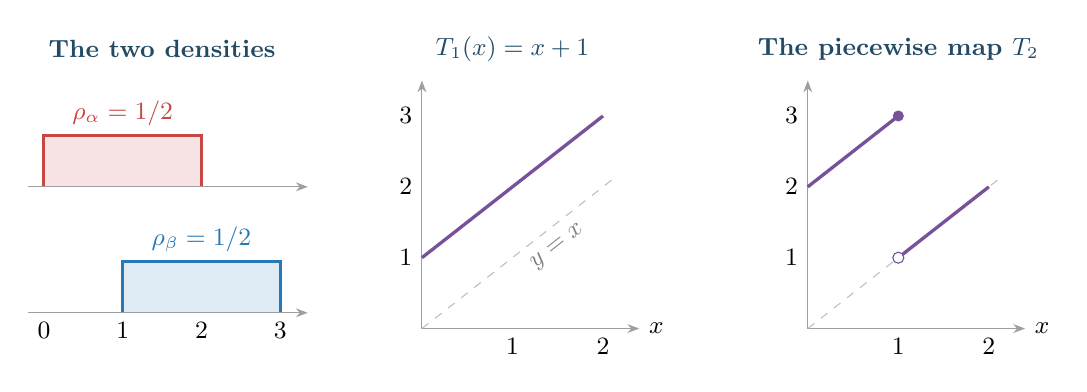
\begin{tikzpicture}[font=\small]
  \node[text=heading,font=\small\bfseries] at (1.5,3.55) {The two densities};
  \fill[sourcecolor!15] (0,1.8) rectangle (2,2.45);
  \draw[exo source] (0,1.8)--(0,2.45)--(2,2.45)--(2,1.8);
  \draw[exo axis] (-.2,1.8)--(3.35,1.8);
  \node[text=sourcecolor,above] at (1,2.45) {$\rho_\alpha=1/2$};
  \fill[targetcolor!15] (1,.2) rectangle (3,.85);
  \draw[exo target] (1,.2)--(1,.85)--(3,.85)--(3,.2);
  \draw[exo axis] (-.2,.2)--(3.35,.2);
  \node[text=targetcolor,above] at (2,.85) {$\rho_\beta=1/2$};
  \foreach \x in {0,1,2,3}{\node[below] at (\x,.2) {$\x$};}
  \begin{scope}[xshift=4.8cm,x=1.15cm,y=.9cm]
    \node[text=heading,font=\small\bfseries] at (1,3.94) {$T_1(x)=x+1$};
    \draw[exo axis] (0,0)--(2.4,0) node[right] {$x$};
    \draw[exo axis] (0,0)--(0,3.5);
    \draw[exo guide] (0,0)--(2.15,2.15);
    \draw[exo map] (0,1)--(2,3);
    \foreach \x in {1,2}{\node[below] at (\x,0) {$\x$};}
    \foreach \y in {1,2,3}{\node[left] at (0,\y) {$\y$};}
    \node[text=gray,rotate=38] at (1.5,1.15) {$y=x$};
  \end{scope}
  \begin{scope}[xshift=9.7cm,x=1.15cm,y=.9cm]
    \node[text=heading,font=\small\bfseries] at (1,3.94) {The piecewise map $T_2$};
    \draw[exo axis] (0,0)--(2.4,0) node[right] {$x$};
    \draw[exo axis] (0,0)--(0,3.5);
    \draw[exo guide] (0,0)--(2.15,2.15);
    \draw[exo map] (0,2)--(1,3);
    \draw[exo map] (1,1)--(2,2);
    \fill[mapcolor] (1,3) circle (2pt);
    \draw[mapcolor,fill=white] (1,1) circle (2pt);
    \foreach \x in {1,2}{\node[below] at (\x,0) {$\x$};}
    \foreach \y in {1,2,3}{\node[left] at (0,\y) {$\y$};}
  \end{scope}
\end{tikzpicture}
\end{center}
\end{exercise}
\begin{hints}
\begin{enumerate}[label=(\roman*)]\item The cost of any admissible map is at least the difference of the means.\item Check the images of the two half-intervals separately, then use $|T(x)-x|=T(x)-x$ when $T(x)\ge x$.\end{enumerate}
\end{hints}
\begin{solution}
\textbf{(i)} Every admissible map satisfies $\int|T(x)-x|\,d\alpha(x)\ge\int(T(x)-x)\,d\alpha(x)=2-1=1$. The translation $T_1(x)=x+1$ has the required image and attains this bound.

\textbf{(ii)} The first half of $[0,2]$ is translated onto $[2,3]$, and the second half is left on $[1,2]$. Both carry density $1/2$, so $T_2$ has image $\beta$. Since $T_2(x)\ge x$, its cost is again $1$.

\end{solution}

\begin{exercise}[Affine images]\label{ex:affine}
(1) \textbf{1-D case.} Let $\mu\in\mathcal P_2(\R)$ and $\nu=(x\mapsto a x+b)_{\push}\mu$ with $a>0$. What is the Monge map from $\mu$ to $\nu$ for the quadratic cost ? Compute the $W_2$ distance in terms of the mean $m_\mu=\int x\,d\mu$ and variance $\mathrm{Var}(\mu)=\int (x-m_\mu)^2\,d\mu$.\\[4pt]
(2) \textbf{Higher dimension.} Let $\mu\in\mathcal P_2(\R^d)$ and $\nu=(x\mapsto A x+b)_{\push}\mu$ with $A\in\mathbb R^{d\times d}$. Give a simple condition on $A$ ensuring that $T(x)=A x+b$ is the Brenier map (assume $\mu$ is absolutely continuous). Under this condition, compute the $W_2$ distance
in terms of $m_\mu=\mathbb E[X]$ and the covariance $\Sigma_\mu=\mathbb E\!\big[(X-m_\mu)(X-m_\mu)^\top\big]$.
\end{exercise}
\begin{hints}
\begin{enumerate}[label=(\arabic*)]\item A positive-slope affine map is increasing. Expand $|(1-a)X-b|^2$ around the mean.\item A symmetric positive-semidefinite matrix gives a convex quadratic potential. Use $\mathbb E\|MX\|^2=\operatorname{tr}(M\Sigma_\mu M^\top)+\|Mm_\mu\|^2$.\end{enumerate}
\end{hints}
\begin{solution}
\emph{(1) 1D.}
Since $a>0$, $x\mapsto ax+b$ is increasing. In 1D the $\Wtwo$--optimal Monge map is the monotone rearrangement, hence $T(x)=ax+b$. Let $X\sim\mu$ with mean $m_\mu$ and variance $\mathrm{Var}(\mu)$. Then
\[
\Wtwo^2(\mu,\nu)=\mathbb E\bigl[(X- (aX+b))^2\bigr]
=\mathbb E\bigl[((1-a)X-b)^2\bigr].
\]
Expand around the mean:
\[
(1-a)X-b=(1-a)(X-m_\mu)+\bigl((1-a)m_\mu-b\bigr),
\]
so the cross term vanishes and
\[
\boxed{\;
\Wtwo^2(\mu,\nu)=(1-a)^2\,\mathrm{Var}(\mu)+\bigl((1-a)m_\mu-b\bigr)^2.\;}
\]

\emph{(2) $\R^d$.}
If $A$ is \textbf{symmetric positive semidefinite}, then there exists a convex quadratic potential $\phi(x)=\tfrac12 x^\top A x+b\cdot x+c$ with $\nabla\phi(x)=Ax+b$. By Brenier, for absolutely continuous $\mu$, $T(x)=Ax+b$ is the unique (a.e.) $\Wtwo$--optimal map.

Let $X\sim\mu$, mean $m_\mu$, covariance $\Sigma_\mu$. Write
\[
X-(AX+b)=(I-A)(X-m_\mu)+\bigl((I-A)m_\mu-b\bigr).
\]
Taking squared norm and expectation, the cross term drops and
\[
\mathbb E\|X-(AX+b)\|^2=\mathrm{tr}\!\bigl((I-A)\Sigma_\mu(I-A)^\top\bigr)+\|(I-A)m_\mu-b\|^2.
\]
Hence
\[
\boxed{\;
\Wtwo^2(\mu,\nu)=\mathrm{tr}\!\bigl((I-A)\Sigma_\mu(I-A)^\top\bigr)+\|(I-A)m_\mu-b\|^2\quad
\text{(for }A\succeq0\text{ symmetric).}\;}
\]

\end{solution}

\begin{exercise}[{Piecewise constant densities on $[0,1]$, quadratic cost}]\label{ex:piecewise}
Let $\alpha$ and $\beta$ have densities
\[
\rho_\alpha(x)=\begin{cases}\frac23,&0\le x<\frac12,\\\frac43,&\frac12\le x\le1,\end{cases}
\qquad
\rho_\beta(x)=\begin{cases}\frac43,&0\le x<\frac12,\\\frac23,&\frac12\le x\le1,\end{cases}
\]
and zero outside $[0,1]$. Construct and sketch the optimal Monge map for the quadratic cost, and compute $\Wtwo^2(\alpha,\beta)$.
\ifcorr\else
\begin{center}
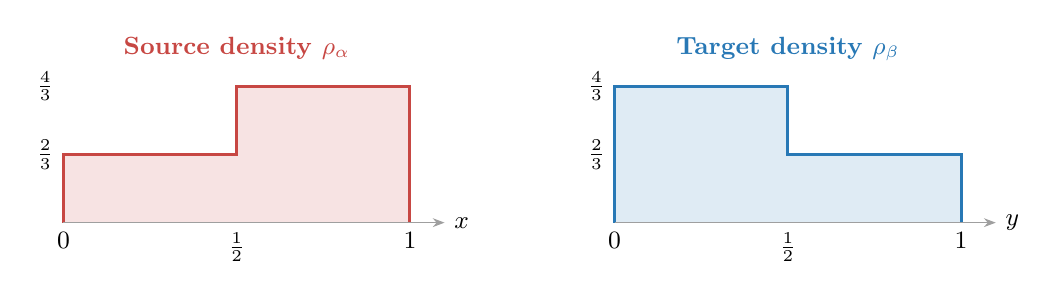
\begin{tikzpicture}[font=\small,x=4.4cm,y=1.3cm]
  \node[text=sourcecolor,font=\small\bfseries] at (.5,1.7) {Source density $\rho_\alpha$};
  \fill[sourcecolor!15] (0,0)--(0,2/3)--(.5,2/3)--(.5,4/3)--(1,4/3)--(1,0)--cycle;
  \draw[exo source] (0,0)--(0,2/3)--(.5,2/3)--(.5,4/3)--(1,4/3)--(1,0);
  \draw[exo axis] (0,0)--(1.1,0) node[right] {$x$};
  \foreach \x/\lab in {0/0,.5/{\tfrac12},1/1}{\node[below] at (\x,0) {$\lab$};}
  \foreach \y/\lab in {.6667/{\tfrac23},1.3333/{\tfrac43}}{\node[left] at (0,\y) {$\lab$};}
  \begin{scope}[xshift=7cm]
    \node[text=targetcolor,font=\small\bfseries] at (.5,1.7) {Target density $\rho_\beta$};
    \fill[targetcolor!15] (0,0)--(0,4/3)--(.5,4/3)--(.5,2/3)--(1,2/3)--(1,0)--cycle;
    \draw[exo target] (0,0)--(0,4/3)--(.5,4/3)--(.5,2/3)--(1,2/3)--(1,0);
    \draw[exo axis] (0,0)--(1.1,0) node[right] {$y$};
    \foreach \x/\lab in {0/0,.5/{\tfrac12},1/1}{\node[below] at (\x,0) {$\lab$};}
    \foreach \y/\lab in {.6667/{\tfrac23},1.3333/{\tfrac43}}{\node[left] at (0,\y) {$\lab$};}
  \end{scope}
\end{tikzpicture}
\end{center}
\fi
\end{exercise}
\begin{hints}
Compute the cumulative functions, and find where the source cumulative crosses the target breakpoint $2/3$. Integrate the squared displacement on the resulting three intervals.
\end{hints}
\begin{solution}
Both densities integrate to $1$. Their cumulative functions satisfy
$C_\alpha(1/2)=1/3$ and $C_\beta(1/2)=2/3$; the latter value is reached by $C_\alpha$ at $x=3/4$.
The optimal map is $T=C_\beta^{-1}\circ C_\alpha$:
\[
T(x)=
\begin{cases}
\dfrac{x}{2}, & x\in[0,\tfrac12],\\[6pt]
x-\dfrac14, & x\in[\tfrac12,\tfrac34],\\[6pt]
2x-1, & x\in[\tfrac34,1].
\end{cases}
\]
The graph consists of three continuous line segments of slopes $1/2,1,2$,
joining $(0,0)$, $(1/2,1/4)$, $(3/4,1/2)$, and $(1,1)$.
\begin{center}
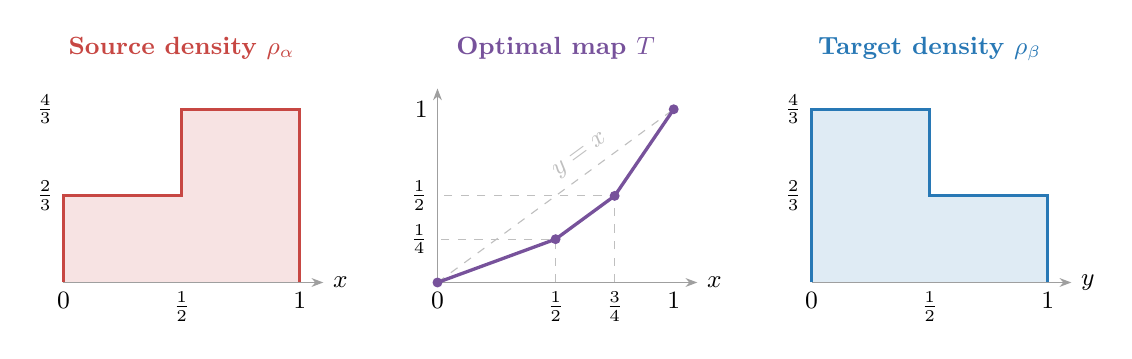
\begin{tikzpicture}[font=\small]
  \begin{scope}[x=3cm,y=1.65cm]
    \node[text=sourcecolor,font=\small\bfseries] at (.5,1.8) {Source density $\rho_\alpha$};
    \fill[sourcecolor!15] (0,0)--(0,2/3)--(.5,2/3)--(.5,4/3)--(1,4/3)--(1,0)--cycle;
    \draw[exo source] (0,0)--(0,2/3)--(.5,2/3)--(.5,4/3)--(1,4/3)--(1,0);
    \draw[exo axis] (0,0)--(1.1,0) node[right] {$x$};
    \foreach \x/\lab in {0/0,.5/{\tfrac12},1/1}{\node[below] at (\x,0) {$\lab$};}
    \foreach \y/\lab in {.6667/{\tfrac23},1.3333/{\tfrac43}}{\node[left] at (0,\y) {$\lab$};}
  \end{scope}
  \begin{scope}[xshift=4.75cm,x=3cm,y=2.2cm]
    \node[text=mapcolor,font=\small\bfseries] at (.5,1.35) {Optimal map $T$};
    \draw[exo axis] (0,0)--(1.1,0) node[right] {$x$};
    \draw[exo axis] (0,0)--(0,1.12);
    \draw[exo guide] (0,0)--(1,1) node[pos=.65,above,sloped] {$y=x$};
    \draw[exo guide] (.5,0)--(.5,.25)--(0,.25);
    \draw[exo guide] (.75,0)--(.75,.5)--(0,.5);
    \draw[exo map] (0,0)--(.5,.25)--(.75,.5)--(1,1);
    \foreach \x/\y in {0/0,.5/.25,.75/.5,1/1}{\fill[mapcolor] (\x,\y) circle (1.8pt);}
    \foreach \x/\lab in {0/0,.5/{\tfrac12},.75/{\tfrac34},1/1}{\node[below] at (\x,0) {$\lab$};}
    \foreach \y/\lab in {.25/{\tfrac14},.5/{\tfrac12},1/1}{\node[left] at (0,\y) {$\lab$};}
  \end{scope}
  \begin{scope}[xshift=9.5cm,x=3cm,y=1.65cm]
    \node[text=targetcolor,font=\small\bfseries] at (.5,1.8) {Target density $\rho_\beta$};
    \fill[targetcolor!15] (0,0)--(0,4/3)--(.5,4/3)--(.5,2/3)--(1,2/3)--(1,0)--cycle;
    \draw[exo target] (0,0)--(0,4/3)--(.5,4/3)--(.5,2/3)--(1,2/3)--(1,0);
    \draw[exo axis] (0,0)--(1.1,0) node[right] {$y$};
    \foreach \x/\lab in {0/0,.5/{\tfrac12},1/1}{\node[below] at (\x,0) {$\lab$};}
    \foreach \y/\lab in {.6667/{\tfrac23},1.3333/{\tfrac43}}{\node[left] at (0,\y) {$\lab$};}
  \end{scope}
\end{tikzpicture}
\end{center}
The cost for the normalized measures is
\[
\frac23\int_0^{1/2}\frac{x^2}{4}\,dx
+\frac43\int_{1/2}^{3/4}\frac1{16}\,dx
+\frac43\int_{3/4}^1(1-x)^2\,dx
=\frac1{144}+\frac1{48}+\frac1{144}=\frac5{144}.
\]
\end{solution}

\begin{exercise}[Translation decomposition for $\Wtwo$]\label{exo:translation}
Let $\alpha,\beta\in\mathcal P_2(\mathbb R^d)$ and assume that $\alpha$ has a Lebesgue density. Throughout this exercise, use the Monge formulation
\[
\Wtwo^2(\alpha,\beta)
=\inf_{S_{\push}\alpha=\beta}\int\|x-S(x)\|^2\,d\alpha(x).
\]
For $u\in\mathbb R^d$ write $T_u(x)=x+u$.

\begin{enumerate}[label=(\alph*), itemsep=4pt]
\item Show there exist unique vectors $a,b$
such that the \emph{centred} measures
\[
\alpha_0:=(T_{-a})_{\push}\alpha,\qquad \beta_0:=(T_{-b})_{\push}\beta
\]
satisfy $\int x\,d\alpha_0(x)=\int x\,d\beta_0(x)=0$, and
\[
\alpha=(T_a)_{\push}\alpha_0,\qquad \beta=(T_b)_{\push}\beta_0.
\]
\item Prove the decomposition
\[
\boxed{\ \Wtwo^2(\alpha,\beta)=\|a-b\|^2+\Wtwo^2(\alpha_0,\beta_0)\ }.
\]
\item If $T_0$ is the Brenier map from $\alpha_0$ to $\beta_0$, show that
\[
T(x):=T_0(x-a)+b
\]
is the Brenier map from $\alpha$ to $\beta$.
\end{enumerate}
\end{exercise}
\begin{hints}
\begin{enumerate}[label=(\alph*)]\item Compute the mean of a translated measure.\item Relate admissible maps by $S(x)=S_0(x-a)+b$. Expand the squared displacement; the mixed term vanishes after integration.\item Use the cost identity in (b). Alternatively, translate the convex potential of $T_0$.\end{enumerate}
\end{hints}
\begin{solution}
\emph{(a) Centring and uniqueness.}
Define $a=\int x\,d\alpha$ and $b=\int x\,d\beta$ (these exist by the $\mathcal P_2$ assumption). Put $\alpha_0=(T_{-a})_{\push}\alpha$. Then, by change of variables,
\[
\int x\,d\alpha_0(x)=\int (x-a)\,d\alpha(x)=\Big(\int x\,d\alpha(x)\Big)-a=0.
\]
Similarly $\int x\,d\beta_0(x)=0$. Also $(T_a)_{\push}\alpha_0=\alpha$ and $(T_b)_{\push}\beta_0=\beta$ by construction. If $\tilde a$ also centres $\alpha$, then $0=\int x\,d(T_{-\tilde a})_{\push}\alpha=\int (x-\tilde a)\,d\alpha=\big(\int x\,d\alpha\big)-\tilde a$, hence $\tilde a=a$; likewise for $b$.

\emph{(b) Decomposition of $\Wtwo^2$.}
There is a bijection between admissible maps for the centred and original measures:
\[
(S_0)_{\push}\alpha_0=\beta_0
\quad\Longleftrightarrow\quad
S_{\push}\alpha=\beta,
\qquad S(x)=S_0(x-a)+b.
\]
Its inverse is $S_0(z)=S(z+a)-b$. Changing variables $x=z+a$ and expanding the square gives
\begin{align*}
\int\|x-S(x)\|^2\,d\alpha(x)
&=\int\|z-S_0(z)+(a-b)\|^2\,d\alpha_0(z)\\
&=\int\|z-S_0(z)\|^2\,d\alpha_0(z)+\|a-b\|^2.
\end{align*}
Indeed, the mixed term vanishes because
$\int(z-S_0(z))\,d\alpha_0(z)=\int z\,d\alpha_0(z)-\int y\,d\beta_0(y)=0$.
The bijection therefore identifies the two infima, with the constant difference $\|a-b\|^2$, which proves (b) directly in the Monge formulation.

\emph{(c) Relation between the optimal maps.}
Both $\alpha$ and its translate $\alpha_0$ have densities, so their Brenier maps exist and are unique almost everywhere. Define $T(x)=T_0(x-a)+b$. Its pushforward is
\[
T_{\push}\alpha=(T_b)_{\push}(T_0)_{\push}(T_{-a})_{\push}\alpha
=(T_b)_{\push}\beta_0=\beta.
\]
By the cost identity in (b),
\[
\int\|x-T(x)\|^2\,d\alpha(x)
=\Wtwo^2(\alpha_0,\beta_0)+\|a-b\|^2=\Wtwo^2(\alpha,\beta),
\]
so $T$ is optimal.

\emph{A second proof, using convex potentials.}
Write $T_0=\nabla\phi_0$ with $\phi_0$ convex. Then
$\phi(x)=\phi_0(x-a)+b\cdot x$ is convex and $\nabla\phi(x)=T(x)$.
Together with $T_{\push}\alpha=\beta$, Brenier's characterization proves optimality directly, without using the cost decomposition in (b).
\end{solution}

\begin{exercise}[Adding separable terms; quadratic cost vs.\ $-\langle x,y\rangle$]\label{ex:add-separable}
Fix $\alpha,\beta\in\mathcal P_2(\mathbb{R}^d)$ and consider Monge maps $T$ with $T_{\push}\alpha=\beta$.

\begin{enumerate}[label=(\alph*), itemsep=4pt]
\item
Let $c:\mathbb{R}^d\times\mathbb{R}^d\to\mathbb{R}$ be a measurable cost and define
$\tilde c(x,y)=c(x,y)+u(x)+v(y)$, with $u:\mathbb{R}^d\to\mathbb{R}$, $v:\mathbb{R}^d\to\mathbb{R}$. Assume $u\in L^1(\alpha)$, $v\in L^1(\beta)$, and that the integral of $c$ is well-defined for every admissible map (for instance $c\ge0$).
Show that the sets of Monge minimizers for $c$ and for $\tilde c$ (with the same marginals) coincide.

\item
Let $\lambda>0$ and define $\hat c(x,y)=\lambda\,c(x,y)$.
Show that the Monge minimizers for $c$ and $\hat c$ coincide.

\item Take
$c_{\mathrm{quad}}(x,y)=\|x-y\|^2,\qquad c_{\mathrm{lin}}(x,y)=-\langle x,y\rangle$.
Prove that $c_{\mathrm{quad}}$ and $c_{\mathrm{lin}}$ have the same Monge minimizers (for fixed $\alpha,\beta$).
\end{enumerate}
\end{exercise}
\begin{hints}
\begin{enumerate}[label=(\alph*)]\item Use $\int v(T(x))\,d\alpha=\int v\,d\beta$.\item A positive multiplier preserves ordering.\item Expand the square and apply the first two parts.\end{enumerate}
\end{hints}
\begin{solution}
\emph{(a) Separable perturbations.}
For any admissible map $T$ with $T_{\push}\alpha=\beta$,
\[
\int \tilde c(x,T(x))\,d\alpha(x)
=\int c(x,T(x))\,d\alpha(x)
+\underbrace{\int u(x)\,d\alpha(x)}_{\text{depends only on }\alpha}
+\underbrace{\int v(y)\,d\beta(y)}_{\text{depends only on }\beta}.
\]
The last two terms are independent of $T$, so the ordering of admissible maps by total cost is the same for $c$ and $\tilde c$. Hence the minimizers coincide.

\emph{(b) Positive rescaling.}
For any admissible $T$,
\[
\int \hat c(x,T(x))\,d\alpha(x)=\lambda\int c(x,T(x))\,d\alpha(x).
\]
Multiplying by $\lambda>0$ preserves the argmin, so the sets of minimizers are the same.

\emph{(c) Quadratic cost vs.\ $-\langle x,y\rangle$.}
Decompose
\[
\|x-y\|^2=\|x\|^2+\|y\|^2-2\langle x,y\rangle
= u(x)+v(y)+\tilde c(x,y),
\]
with $u(x)=\|x\|^2$, $v(y)=\|y\|^2$, and $\tilde c(x,y)=-2\langle x,y\rangle$.
By part (a), $c_{\mathrm{quad}}$ and $\tilde c$ have the same Monge minimizers.
By part (b), $\tilde c=-2\langle x,y\rangle$ and $c_{\mathrm{lin}}=-\langle x,y\rangle$ have the same minimizers as well (rescaling by $2>0$). Consequently, the Monge minimizers for
\[
c_{\mathrm{quad}}(x,y)=\|x-y\|^2
\quad\text{and}\quad
c_{\mathrm{lin}}(x,y)=-\langle x,y\rangle
\]
coincide.

\smallskip
\emph{Remark (value relation).} For any admissible $T$,
\[
\int\|x-T(x)\|^2\,d\alpha
=\int\|x\|^2\,d\alpha+\int\|y\|^2\,d\beta-2\int\langle x,T(x)\rangle\,d\alpha,
\]
so minimizing the quadratic cost is equivalent to maximizing the correlation term $\int\langle x,T(x)\rangle\,d\alpha$; the optimal \emph{map} is the same in both problems, although the optimal \emph{values} differ by the constants depending only on $\alpha,\beta$.
\end{solution}

\begin{exercise}[Quantile coupling: explicit computation]\label{ex:quantile}
Let $\alpha=\Unif[0,1]$ and let $\beta$ be supported on $[0,1]$ with density $\rho_\beta(y)=2y$.
\begin{enumerate}[label=(\alph*)]
\item Compute the cumulative functions $C_\alpha,C_\beta$ and their quantiles $C_\alpha^{-1},C_\beta^{-1}$.
\item Using monotone transport in 1D, write the optimal map $T=C_\beta^{-1}\circ C_\alpha$.
\item Compute $\Wtwo^2(\alpha,\beta)$ using both $\int_0^1|x-T(x)|^2\,dx$ and the quantile formula $\int_0^1|C_\alpha^{-1}(r)-C_\beta^{-1}(r)|^2\,dr$.
\end{enumerate}
\begin{center}
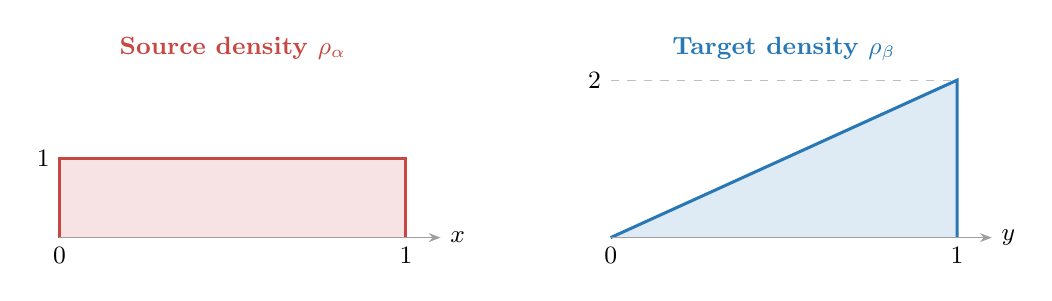
\begin{tikzpicture}[font=\small,x=4.4cm,y=1cm]
  \node[text=sourcecolor,font=\small\bfseries] at (.5,2.4) {Source density $\rho_\alpha$};
  \fill[sourcecolor!15] (0,0) rectangle (1,1);
  \draw[exo source] (0,0)--(0,1)--(1,1)--(1,0);
  \draw[exo axis] (0,0)--(1.1,0) node[right] {$x$};
  \node[left] at (0,1) {$1$};
  \foreach \x in {0,1}{\node[below] at (\x,0) {$\x$};}
  \begin{scope}[xshift=7cm]
    \node[text=targetcolor,font=\small\bfseries] at (.5,2.4) {Target density $\rho_\beta$};
    \fill[targetcolor!15] (0,0)--(1,2)--(1,0)--cycle;
    \draw[exo target] (0,0)--(1,2)--(1,0);
    \draw[exo axis] (0,0)--(1.1,0) node[right] {$y$};
    \draw[exo guide] (0,2)--(1,2);
    \node[left] at (0,2) {$2$};
    \foreach \x in {0,1}{\node[below] at (\x,0) {$\x$};}
  \end{scope}
\end{tikzpicture}
\end{center}
\end{exercise}
\begin{hints}
\begin{enumerate}[label=(\alph*)]\item Integrate $2y$ from $0$ to $y$, then invert.\item Compose the target quantile with the source cumulative.\item Expand $(x-\sqrt{x})^2$ and integrate its three terms.\end{enumerate}
\end{hints}
\begin{solution}
\textbf{(a)} On $[0,1]$, $C_\alpha(x)=x$ and $C_\beta(x)=x^2$. Both cumulative functions are $0$ to the left of the interval and $1$ to its right. Their quantiles are $C_\alpha^{-1}(r)=r$ and $C_\beta^{-1}(r)=\sqrt r$ for $0<r<1$, with the continuous endpoint extensions $0,1$.

\textbf{(b)} Since the source cumulative is the identity on $[0,1]$, the optimal map is $T(x)=C_\beta^{-1}(C_\alpha(x))=\sqrt{x}$.
\begin{center}
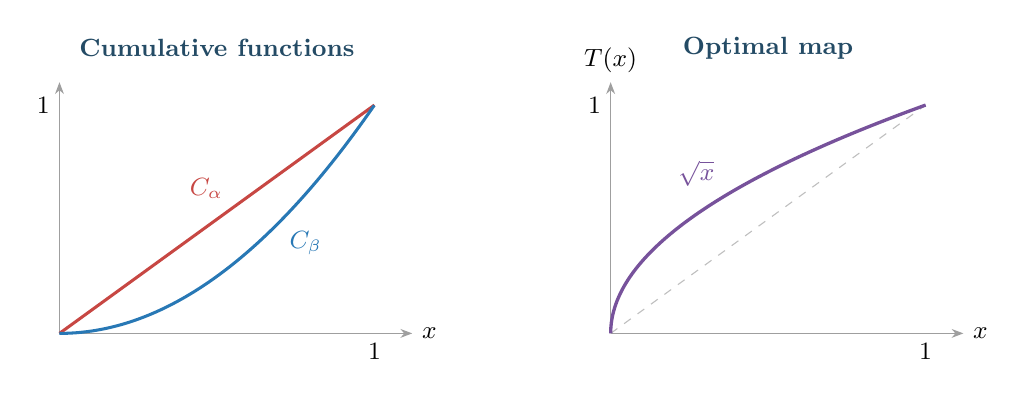
\begin{tikzpicture}[font=\small,x=4cm,y=2.9cm]
  \node[text=heading,font=\small\bfseries] at (.5,1.25) {Cumulative functions};
  \draw[exo axis] (0,0)--(1.12,0) node[right] {$x$};
  \draw[exo axis] (0,0)--(0,1.1);
  \draw[exo source] (0,0)--(1,1);
  \draw[exo target,domain=0:1,samples=60] plot (\x,{\x*\x});
  \node[text=sourcecolor,above left] at (.55,.55) {$C_\alpha$};
  \node[text=targetcolor,below right] at (.7,.49) {$C_\beta$};
  \node[left] at (0,1) {$1$}; \node[below] at (1,0) {$1$};
  \begin{scope}[xshift=7cm]
    \node[text=heading,font=\small\bfseries] at (.5,1.25) {Optimal map};
    \draw[exo axis] (0,0)--(1.12,0) node[right] {$x$};
    \draw[exo axis] (0,0)--(0,1.1) node[above] {$T(x)$};
    \draw[exo guide] (0,0)--(1,1);
    \draw[exo map,domain=0:1,samples=65,variable=\t] plot ({\t*\t},\t);
    \node[text=mapcolor,above left] at (.36,.6) {$\sqrt x$};
    \node[left] at (0,1) {$1$}; \node[below] at (1,0) {$1$};
  \end{scope}
\end{tikzpicture}
\end{center}
\textbf{(c)} Expanding the squared displacement gives
\[
\Wtwo^2(\alpha,\beta)
=\int_0^1(x-\sqrt x)^2\,dx
=\frac13-\frac45+\frac12=\frac1{30}.
\]
The quantile formula gives the same integral, with the probability variable $r$ in place of $x$.
\end{solution}

\begin{exercise}[Cumulative functions]\label{ex:PIT}
Let $\alpha$ be a probability measure on $\mathbb{R}$ and let its cumulative distribution function be
\[
C_\alpha(x)=\alpha\bigl((-\infty,x]\bigr),\qquad x\in\mathbb{R}.
\]
Consider the pushforward by $C_\alpha$, namely $(C_\alpha)_{\push}\alpha$.

\begin{itemize}[itemsep=2pt]
\item[(1)] Assume $\alpha$ is atomless (equivalently, $C_\alpha$ is continuous). This includes, but is not restricted to, measures with a Lebesgue density. Prove that
\[
(C_\alpha)_{\push}\alpha=\Unif[0,1].
\]
In your proof, clearly point out \emph{where} the continuity assumption is used.
\item[(2)] What happens if $\alpha$ is purely discrete, say $\alpha=\sum_{i} p_i\,\delta_{x_i}$ with $\sum_i p_i=1$ and $x_1<x_2<\cdots$? Describe the law of $C_\alpha(X)$ for $X\sim\alpha$, and show that for all $t\in[0,1]$,
\[
\mathbb{P}\bigl(C_\alpha(X)\le t\bigr)\le t,
\]
with equality at the jump values of $C_\alpha$.
\end{itemize}
\end{exercise}
\begin{hints}
\begin{enumerate}[label=(\arabic*)]\item If $U$ is uniform on $(0,1)$, then $C_\alpha^{-1}(U)$ has law $\alpha$. Use continuity to evaluate $C_\alpha(C_\alpha^{-1}(u))$.\item At $x_i$ the cumulative is the partial sum $s_i=\sum_{j\le i}p_j$. Sum exactly those masses with $s_i\le t$.\end{enumerate}
\end{hints}
\begin{solution}
\textbf{(1)} Write $F=C_\alpha$ and $Q(u)=\inf\{x:F(x)\ge u\}$ for $0<u<1$. For $U\sim\Unif(0,1)$, the equivalence $Q(U)\le x\iff U\le F(x)$ proves $Q(U)\sim\alpha$. Continuity of $F$ gives $F(Q(u))=u$ for $0<u<1$, even when $F$ has flat intervals. Consequently $F(Q(U))=U$ almost surely, so $F_\#\alpha=\Unif[0,1]$.

Continuity excludes jumps, not flat intervals. It is equivalent to absence of atoms, not to existence of a density; a singular atomless law also satisfies the conclusion. Endpoints $u=0,1$ are null events and need no finite quantile convention.

\textbf{(2)} At the ordered atoms, $F(x_i)=s_i$, so
\[
F_\#\alpha=\sum_i p_i\delta_{s_i},\qquad
\mathbb P(F(X)\le t)=\sum_{i:s_i\le t}p_i\le t.
\]
For a finite initial segment the sum equals its last partial sum; for an infinite one take a limit. Equality holds at $t=s_i$ (and at $0,1$). Thus the image measure is \emph{discrete}: it puts mass $p_i$ at the cumulative mass $s_i$, independently of the locations $x_i$. It is not uniform. Its cumulative lies below the uniform cumulative, a property often called \emph{super-uniformity}.

How far is this law from uniform? Put $s_0=0$ and $H(t)=\mathbb P(F(X)\le t)$. On each interval $[s_{i-1},s_i)$, $H(t)=s_{i-1}$, so
\[
\sup_{0\le t\le1}|H(t)-t|=\sup_i p_i,
\qquad
\Wone(F_{\push}\alpha,\Unif[0,1])=\frac12\sum_i p_i^2.
\]
The first quantity is the Kolmogorov--Smirnov distance. For the second, the increasing map from a uniform variable sends $(s_{i-1},s_i]$ to $s_i$; its cost on that interval is $\int_{s_{i-1}}^{s_i}(s_i-r)\,dr=p_i^2/2$.

For example, take $n\ge2$ equispaced points $x_i=(i-1)/(n-1)$ in $[0,1]$, each with mass $1/n$. Then
\[
\alpha=\frac1n\sum_{i=1}^n\delta_{(i-1)/(n-1)},
\qquad
F_{\push}\alpha=\frac1n\sum_{i=1}^n\delta_{i/n}.
\]
The image law is uniform on the \emph{finite grid} $\{1/n,2/n,\ldots,1\}$. Its Kolmogorov--Smirnov distance to $\Unif[0,1]$ is $1/n$, and its $\Wone$ distance is $1/(2n)$. It therefore converges weakly to the continuous uniform law, although each image measure is purely atomic.
\end{solution}

\begin{exercise}[Pushforward of a uniform law by a nonlinear map]\label{ex:square}
Let $\alpha=\Unif[-1,1]$ and consider the map $T:\R\to\R$, $T(x)=x^2$.
\begin{itemize}[itemsep=2pt]
\item[(1)] Compute the law $\beta=T_{\push}\alpha$, i.e.\ find its density with respect to Lebesgue measure.
\item[(2)] Check that this density integrates to $1$ over its support.
\item[(3)] Sketch the graph of the density and comment on its behaviour near $0$ and $1$.
\end{itemize}
\ifcorr\else
\begin{center}
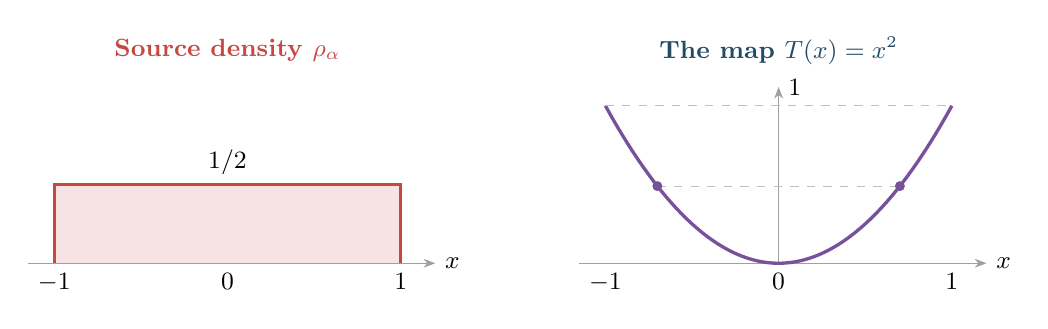
\begin{tikzpicture}[font=\small,x=2.2cm,y=2cm]
  \node[text=sourcecolor,font=\small\bfseries] at (0,1.35) {Source density $\rho_\alpha$};
  \fill[sourcecolor!15] (-1,0) rectangle (1,.5);
  \draw[exo source] (-1,0)--(-1,.5)--(1,.5)--(1,0);
  \draw[exo axis] (-1.15,0)--(1.2,0) node[right] {$x$};
  \node[above] at (0,.5) {$1/2$};
  \foreach \x in {-1,0,1}{\node[below] at (\x,0) {$\x$};}
  \begin{scope}[xshift=7cm]
    \node[text=heading,font=\small\bfseries] at (0,1.35) {The map $T(x)=x^2$};
    \draw[exo axis] (-1.15,0)--(1.2,0) node[right] {$x$};
    \draw[exo axis] (0,0)--(0,1.12);
    \draw[exo map,domain=-1:1,samples=65] plot (\x,{\x*\x});
    \draw[exo guide] (-1,1)--(1,1);
    \draw[exo guide] (-.7,.49)--(.7,.49);
    \fill[mapcolor] (-.7,.49) circle (1.8pt);
    \fill[mapcolor] (.7,.49) circle (1.8pt);
    \node[above right] at (0,1) {$1$};
    \foreach \x in {-1,0,1}{\node[below] at (\x,0) {$\x$};}
  \end{scope}
\end{tikzpicture}
\end{center}
\fi
\end{exercise}
\begin{hints}
\begin{enumerate}[label=(\arabic*)]\item Compute $\mathbb P(X^2\le y)$ before differentiating, or add the contributions from $\pm\sqrt y$.\item Use the antiderivative $\sqrt y$.\item Distinguish an integrable density singularity from an atom.\end{enumerate}
\end{hints}
\begin{solution}
(1) Let $X\sim\Unif[-1,1]$ with density $\rho_\alpha(x)=\tfrac12$ on $[-1,1]$.
Define $Y=T(X)=X^2$. Then $Y$ takes values in $[0,1]$.
For $y\in(0,1)$, the preimage under $T$ is $\{\pm \sqrt{y}\}$. By the standard change-of-variable formula for densities,
\[
\rho_\beta(y)=\sum_{x:\,x^2=y} \frac{\rho_\alpha(x)}{|T'(x)|}.
\]
Here $T'(x)=2x$, so $|T'(\pm\sqrt y)|=2\sqrt y$. Each preimage contributes
\[
\frac{\rho_\alpha(\pm\sqrt y)}{|T'(\pm\sqrt y)|}=\frac{1/2}{2\sqrt y}=\frac{1}{4\sqrt y}.
\]
Summing over $\pm\sqrt y$,
\[
\rho_\beta(y)=\frac{1}{4\sqrt y}+\frac{1}{4\sqrt y}=\frac{1}{2\sqrt y},\qquad y\in(0,1].
\]
Thus
\[
\boxed{\;\rho_\beta(y)=\frac{1}{2\sqrt y}\ \text{ for } y\in(0,1],\quad \rho_\beta(y)=0\ \text{ otherwise.}\;}
\]

(2) Check normalization:
\[
\int_0^1 \frac{1}{2\sqrt y}\,dy
=\left[ \sqrt y \,\right]_{0}^1
=1.
\]
So $\rho_\beta$ is a valid density. Equivalently, its cumulative on $[0,1]$ is $C_\beta(y)=\sqrt y$.

(3) The density diverges like $1/(2\sqrt y)$ as $y\downarrow0$, because the squaring map compresses lengths near the origin and both branches contribute. This is an integrable singularity, not an atom: $\beta(\{0\})=\alpha(\{0\})=0$. The density decreases to $1/2$ at $y=1$.
\begin{center}
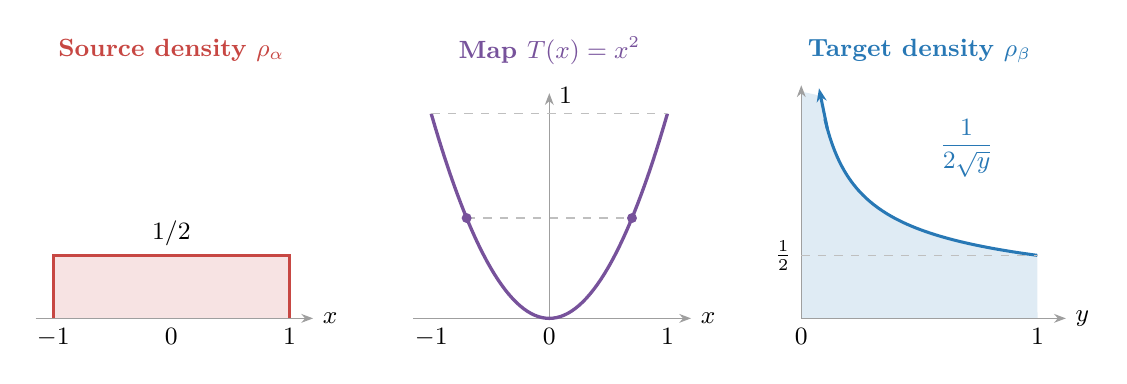
\begin{tikzpicture}[font=\small]
  \begin{scope}[x=1.5cm,y=1.6cm]
    \node[text=sourcecolor,font=\small\bfseries] at (0,2.125) {Source density $\rho_\alpha$};
    \fill[sourcecolor!15] (-1,0) rectangle (1,.5);
    \draw[exo source] (-1,0)--(-1,.5)--(1,.5)--(1,0);
    \draw[exo axis] (-1.15,0)--(1.2,0) node[right] {$x$};
    \node[above] at (0,.5) {$1/2$};
    \foreach \x in {-1,0,1}{\node[below] at (\x,0) {$\x$};}
  \end{scope}
  \begin{scope}[xshift=4.8cm,x=1.5cm,y=2.6cm]
    \node[text=mapcolor,font=\small\bfseries] at (0,1.3077) {Map $T(x)=x^2$};
    \draw[exo axis] (-1.15,0)--(1.2,0) node[right] {$x$};
    \draw[exo axis] (0,0)--(0,1.1);
    \draw[exo map,domain=-1:1,samples=65] plot (\x,{\x*\x});
    \draw[exo guide] (-1,1)--(1,1);
    \draw[exo guide] (-.7,.49)--(.7,.49);
    \fill[mapcolor] (-.7,.49) circle (1.8pt);
    \fill[mapcolor] (.7,.49) circle (1.8pt);
    \node[above right] at (0,1) {$1$};
    \foreach \x in {-1,0,1}{\node[below] at (\x,0) {$\x$};}
  \end{scope}
  \begin{scope}[xshift=8cm,x=3cm,y=1.6cm]
    \node[text=targetcolor,font=\small\bfseries] at (.5,2.125) {Target density $\rho_\beta$};
    \fill[targetcolor!15,domain=.08:1,samples=90]
      (0,0)--(0,1.8)--plot (\x,{.5/sqrt(\x)})--(1,0)--cycle;
    \draw[exo target,domain=.1:1,samples=90] plot (\x,{.5/sqrt(\x)});
    \draw[exo target,-{Stealth[length=1.7mm]}] (.11,1.508)--(.075,1.826);
    \draw[exo axis] (0,0)--(1.12,0) node[right] {$y$};
    \draw[exo axis] (0,0)--(0,1.85);
    \draw[exo guide] (0,.5)--(1,.5);
    \node[left] at (0,.5) {$\tfrac12$};
    \node[below] at (0,0) {$0$}; \node[below] at (1,0) {$1$};
    \node[text=targetcolor] at (.7,1.35) {$\dfrac1{2\sqrt y}$};
  \end{scope}
\end{tikzpicture}
\end{center}
\end{solution}

\Needspace{14\baselineskip}
\section*{Further exercises}

\begin{exercise}[Radial symmetry]\label{ex:radial}
Let $\alpha,\beta\in\mathcal P_2(\R^d)$ be invariant under all orthogonal maps, and assume $\alpha$ is absolutely continuous. Define the radial cumulative function
$F_\mu(r)=\mu(\{x:\|x\|\le r\})$, $r\ge0$, and its generalized inverse for $0<u<1$.
\begin{enumerate}[label=(\roman*)]
\item Show that the unique quadratic optimal map commutes with orthogonal maps: $Q\circ T\circ Q^{-1}=T$ $\alpha$-a.e. Show that it has a radial representative $T(x)=t(\|x\|)x/\|x\|$ for $\alpha$-a.e. $x\ne0$, with $t$ nonnegative and nondecreasing on the relevant radii.
\item Prove $t(r)=F_\beta^{-1}(F_\alpha(r))$ for almost every source radius. Does $F_\beta(t(r))=F_\alpha(r)$ still hold if $\beta$ has an atom on a sphere?
\item Specialize to uniform laws on balls of positive radii $R_\alpha,R_\beta$. Give the map and its squared cost.
\end{enumerate}
\end{exercise}
\begin{hints}
\begin{enumerate}[label=(\roman*)]
\item Conjugate an optimal map by $Q$ and use uniqueness. To avoid choosing exceptional sets for all $Q$ simultaneously, construct a radial optimizer directly using $\|x-y\|\ge|\|x\|-\|y\||$.
\item Apply one-dimensional increasing rearrangement to the laws of the radii. The target radial cumulative may have jumps.
\item The source radial cumulative is $(r/R_\alpha)^d$. Compute $\mathbb E\|X\|^2$ in polar coordinates.
\end{enumerate}
\end{hints}
\begin{solution}
\textbf{(i)} Orthogonal invariance of the marginals and cost makes $Q\circ T\circ Q^{-1}$ another optimizer. Brenier uniqueness gives the stated equality for each fixed $Q$.

For a direct construction, let $R=\|X\|$ for $X\sim\alpha$. Its law is atomless. By radial invariance, $X=RU$ where $U$ is uniform on the unit sphere and independent of $R$ (in dimension one the sphere consists of $\{-1,1\}$). Put $t=F_\beta^{-1}\circ F_\alpha$. Then $t(R)$ has the target radial law, and $t(R)U$ has law $\beta$, including any target mass at the origin.

Every coupling of $\alpha,\beta$ induces a coupling of their radii and satisfies
\[
\int\|x-y\|^2\,d\pi\ge\int|\|x\|-\|y\||^2\,d\pi
\ge\int|r-t(r)|^2\,d(\|\cdot\|_\#\alpha)(r).
\]
The constructed map attains both inequalities. It is therefore the unique optimal map, with the claimed radial form. Its radial profile is nonnegative and nondecreasing. The value at $x=0$ may be set arbitrarily since $\alpha(\{0\})=0$.

\textbf{(ii)} The preceding construction proves the quantile formula. More precisely, for $u=F_\alpha(r)\in(0,1)$,
\[
F_\beta(t(r)^-)\le u\le F_\beta(t(r)).
\]
Equality on the right requires continuity at the target radius and is false in general: if $\beta$ is uniform on the unit sphere, then $t(r)=1$ for almost every source radius, while $F_\beta(1)=1$. Mass conservation means $t_\#(\|\cdot\|_\#\alpha)=\|\cdot\|_\#\beta$, not a pointwise equality of cumulative functions at jumps.

\textbf{(iii)} For uniform balls, matching $(r/R_\alpha)^d$ with $(t/R_\beta)^d$ gives $T(x)=(R_\beta/R_\alpha)x$. Since $\mathbb E\|X\|^2=dR_\alpha^2/(d+2)$,
\[
\Wtwo^2(\alpha,\beta)=\frac{d}{d+2}(R_\alpha-R_\beta)^2.
\]
This also follows directly because a positive dilation is the gradient of a convex quadratic.
\end{solution}


\end{document}
